\begin{frame}{Final Experimental Setup}
\begin{table}
\centering
\small
\begin{tabular}{ll}
\toprule
Item & Setting \\
\midrule
Task & Binary fake review detection \\
Dataset & \texttt{testing/data/deepseek\_synthetic\_reviews.jsonl} \\
Model & \texttt{answerdotai/ModernBERT-large} \\
Train/eval split & 90/10, seed 42 \\
Training & 5 epochs, batch size 8, grad. accumulation 4 \\
Methods & Full, LoRA, AdaLoRA, Star-LoRA \\
Metrics & F1, eval loss, runtime, throughput \\
\bottomrule
\end{tabular}
\end{table}
\end{frame}

\begin{frame}{Baselines and Star-LoRA Configuration}
\begin{table}
\centering
\scriptsize
\begin{tabular}{lccccc}
\toprule
Method & Targets & Rank & Init rank & Alpha & Dropout \\
\midrule
LoRA & Wqkv, Wo & 8 & -- & 16 & 0.10 \\
AdaLoRA baseline & Wqkv, Wo & 8 & 12 & 16 & 0.10 \\
Star-LoRA & Wqkv, Wo & 12 & 24 & 48 & 0.05 \\
\bottomrule
\end{tabular}
\end{table}

\vspace{6pt}
\begin{itemize}
  \item AdaLoRA baseline uses a reasonable manual setting, not a guaranteed tuned optimum.
  \item Star-LoRA selected a larger capacity from the full training set statistics.
  \item Recorded dataset statistics: balanced labels, token sparsity \(0.450\), label entropy \(\approx 1.0\).
  \item Target modules are fixed for fair ModernBERT comparison; capacity settings are dataset-aware.
\end{itemize}
\end{frame}

\begin{frame}{AdaLoRA Baseline Setting}
\small
\begin{itemize}
  \item Manual AdaLoRA baseline:
  \[
    r_{\mathrm{target}}=8,\quad
    r_{\mathrm{init}}=12,\quad
    \alpha=16,\quad
    p_{\mathrm{drop}}=0.10.
  \]
  \item \(r_{\mathrm{init}}>r_{\mathrm{target}}\): AdaLoRA starts with extra rank and prunes/reallocates during training.
  \item \(\alpha\): scaling strength of adapter update.
  \item \(p_{\mathrm{drop}}\): regularization for adapter inputs.
  \item This baseline is manually configured AdaLoRA, not best possible tuned AdaLoRA.
\end{itemize}
\end{frame}

\begin{frame}{Final Full-Data Results}
\begin{figure}
    \centering
    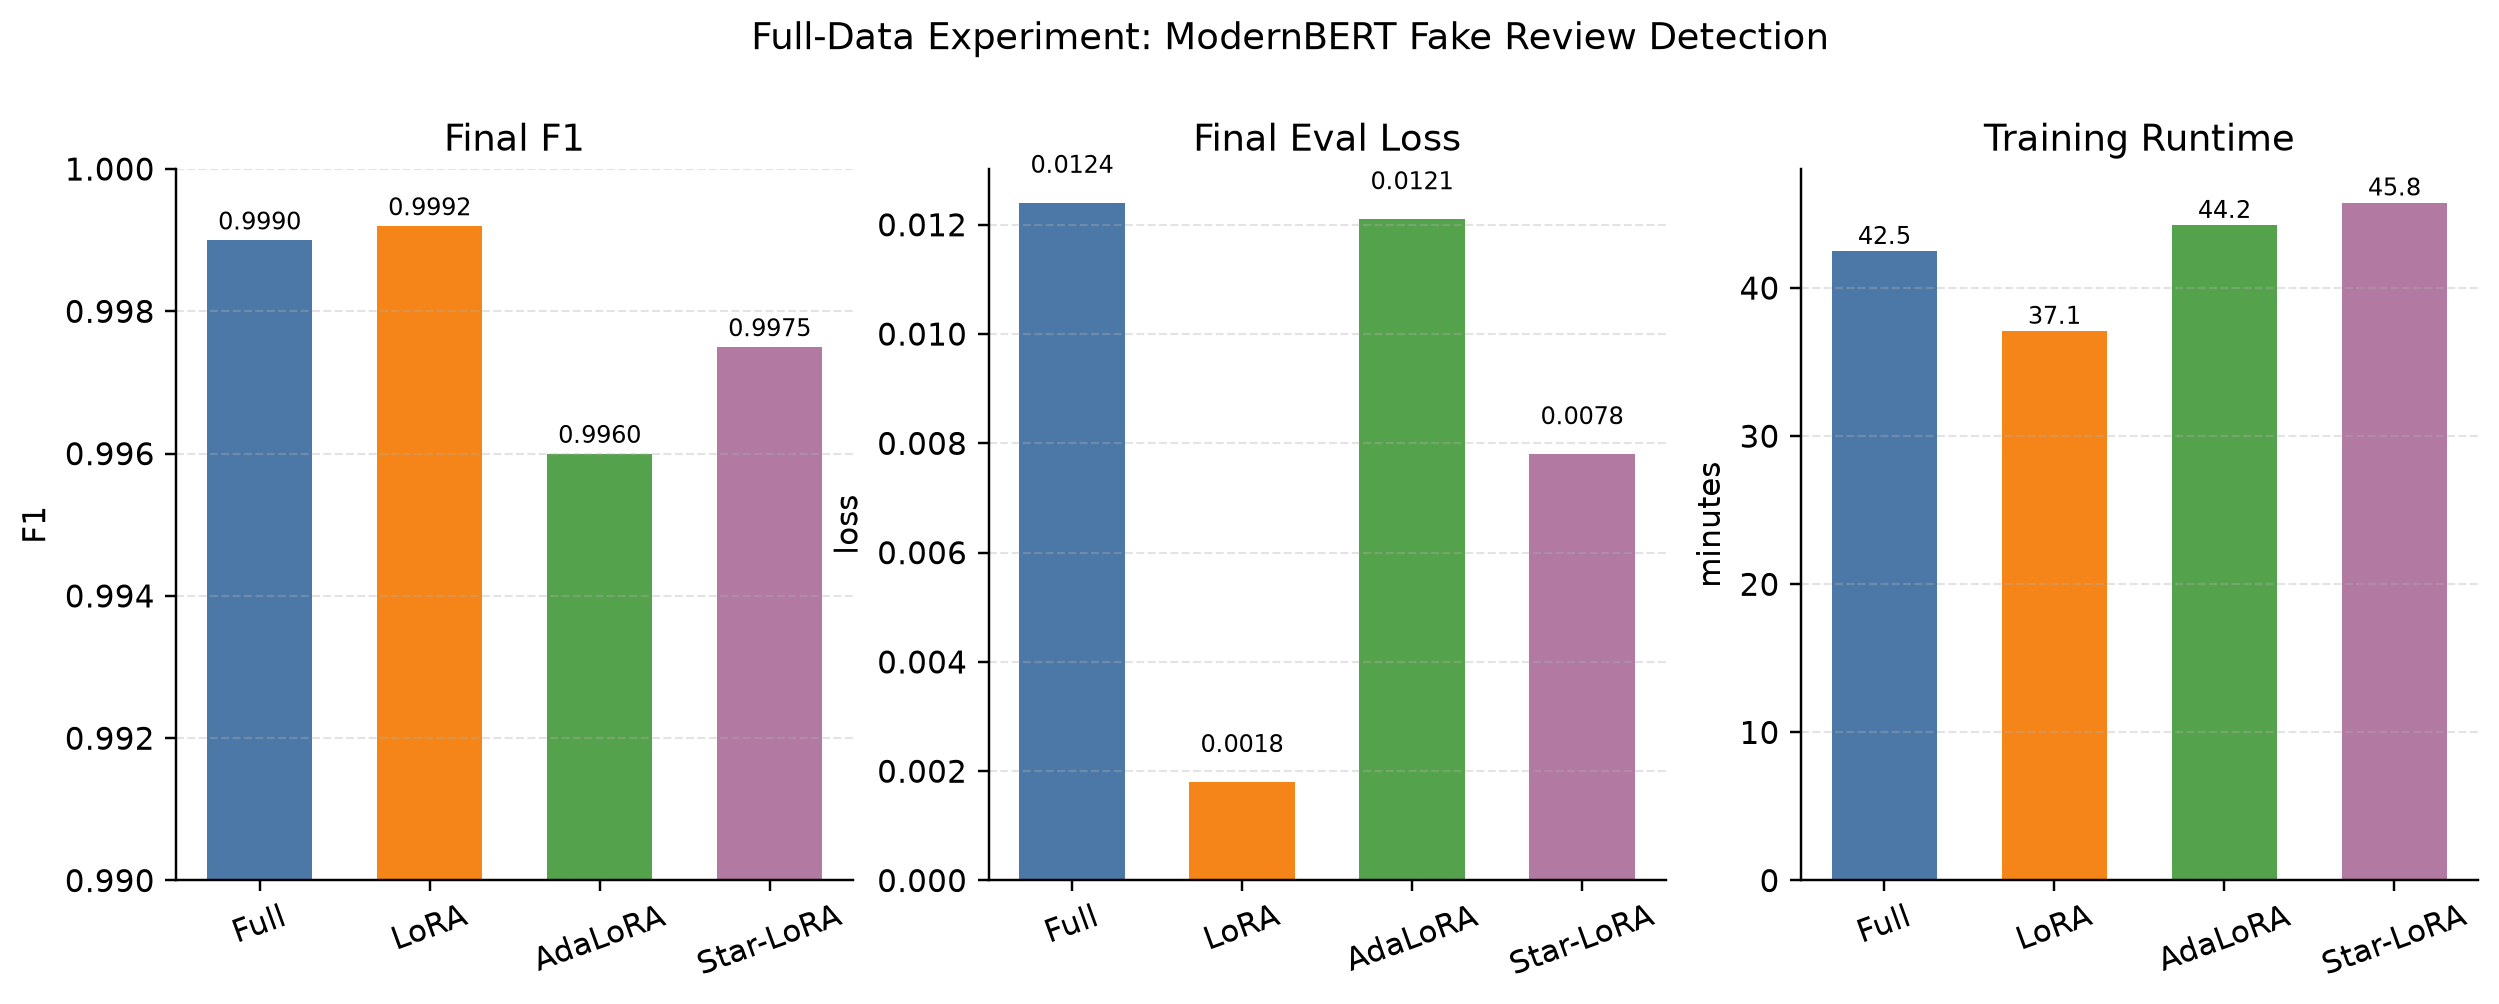
\includegraphics[width=0.96\linewidth]{figures/final_summary.png}
\end{figure}
\end{frame}

\begin{frame}{Final Metrics Table}
\begin{table}
\centering
\scriptsize
\begin{tabular}{lrrrr}
\toprule
Method & Final F1 & Eval loss & Runtime (s) & Samples/s \\
\midrule
Full & 0.9990 & 0.0124 & 2548.62 & 70.63 \\
LoRA & \textbf{0.9992} & \textbf{0.0018} & \textbf{2225.13} & \textbf{80.89} \\
AdaLoRA & 0.9960 & 0.0121 & 2654.11 & 67.82 \\
Star-LoRA & 0.9975 & 0.0078 & 2745.00 & 65.57 \\
\bottomrule
\end{tabular}
\end{table}

\vspace{6pt}
\begin{itemize}
  \item Star-LoRA improves over AdaLoRA on the final full-data run.
  \item Fixed LoRA remains the strongest result on this dataset.
\end{itemize}
\end{frame}

\begin{frame}{Data-Size Sweep}
\begin{figure}
    \centering
    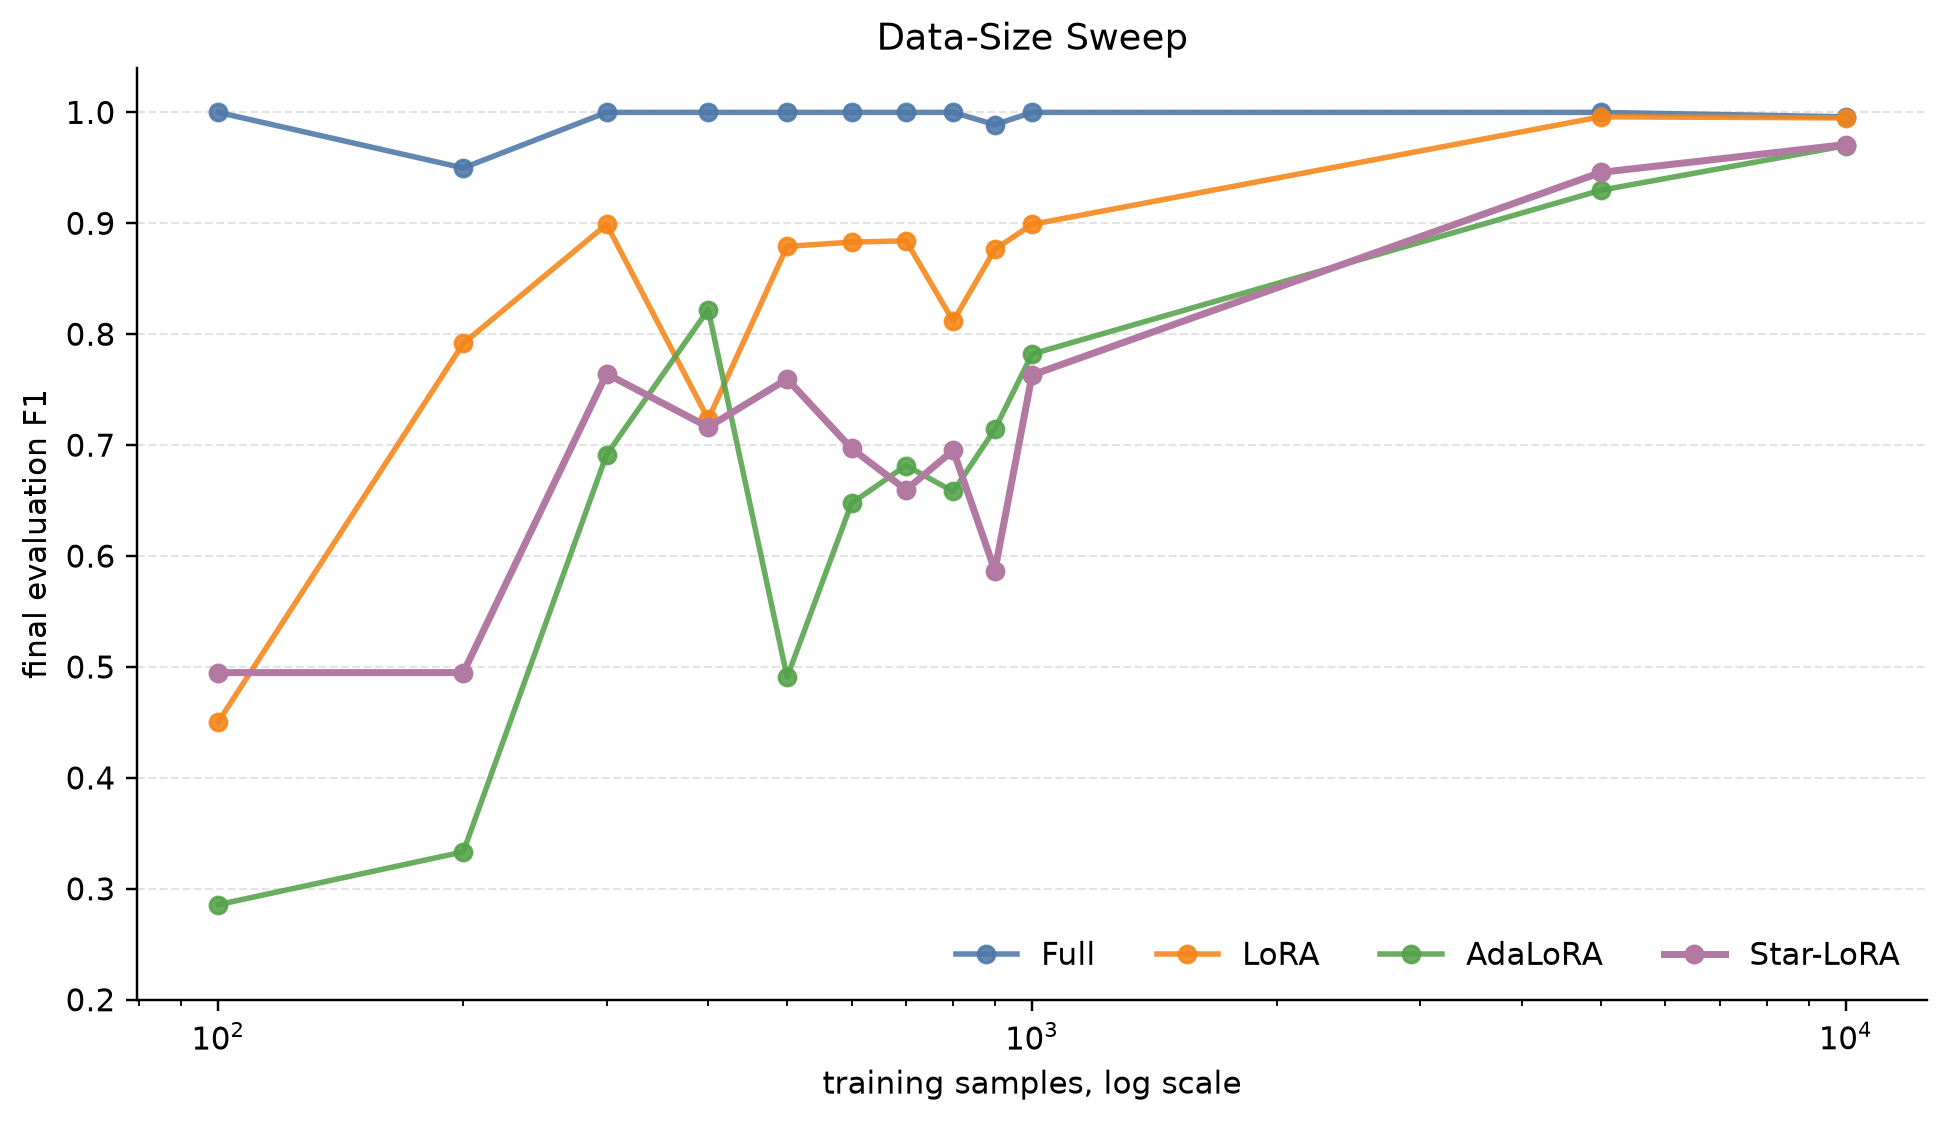
\includegraphics[width=0.93\linewidth]{figures/datasize_f1_logx.png}
\end{figure}
\end{frame}

\begin{frame}{Where Star-LoRA Helps}
\begin{figure}
    \centering
    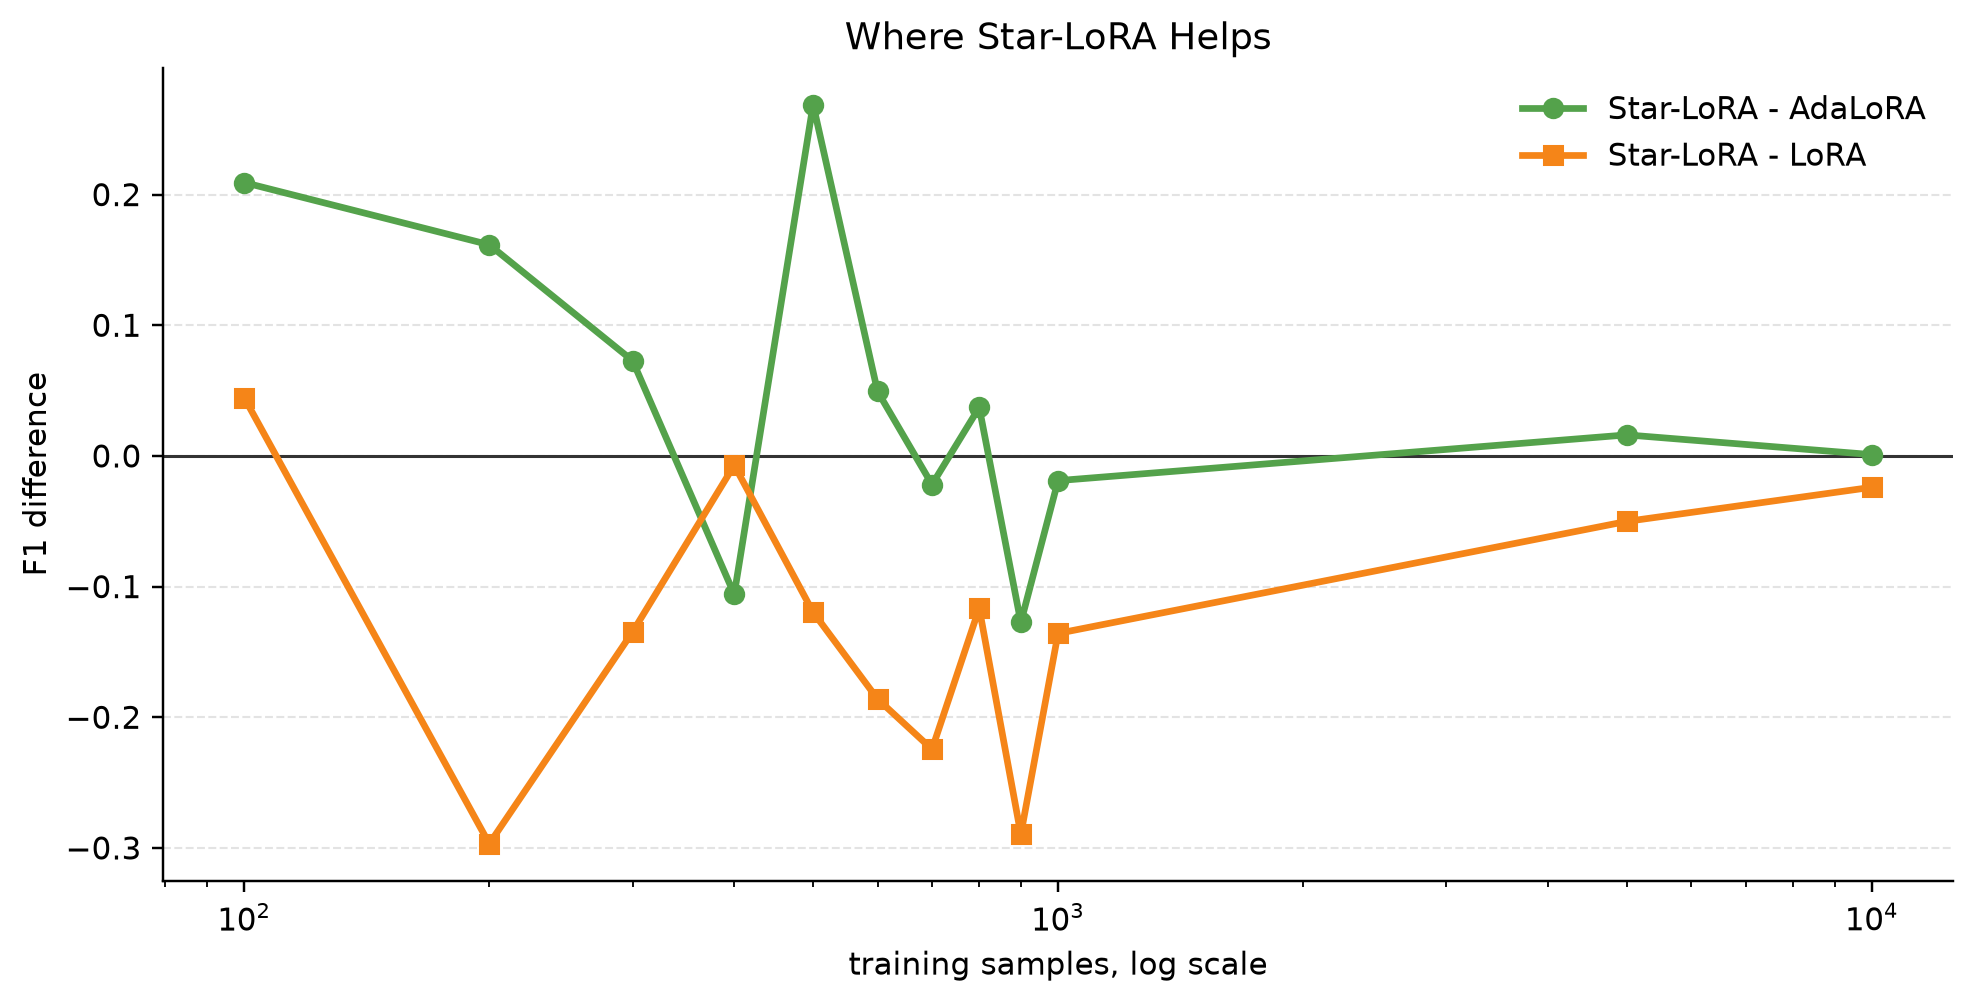
\includegraphics[width=0.93\linewidth]{figures/star_lora_delta.png}
\end{figure}
\end{frame}

\begin{frame}{Dataset-Aware Capacity Selected by Star-LoRA}
\begin{figure}
    \centering
    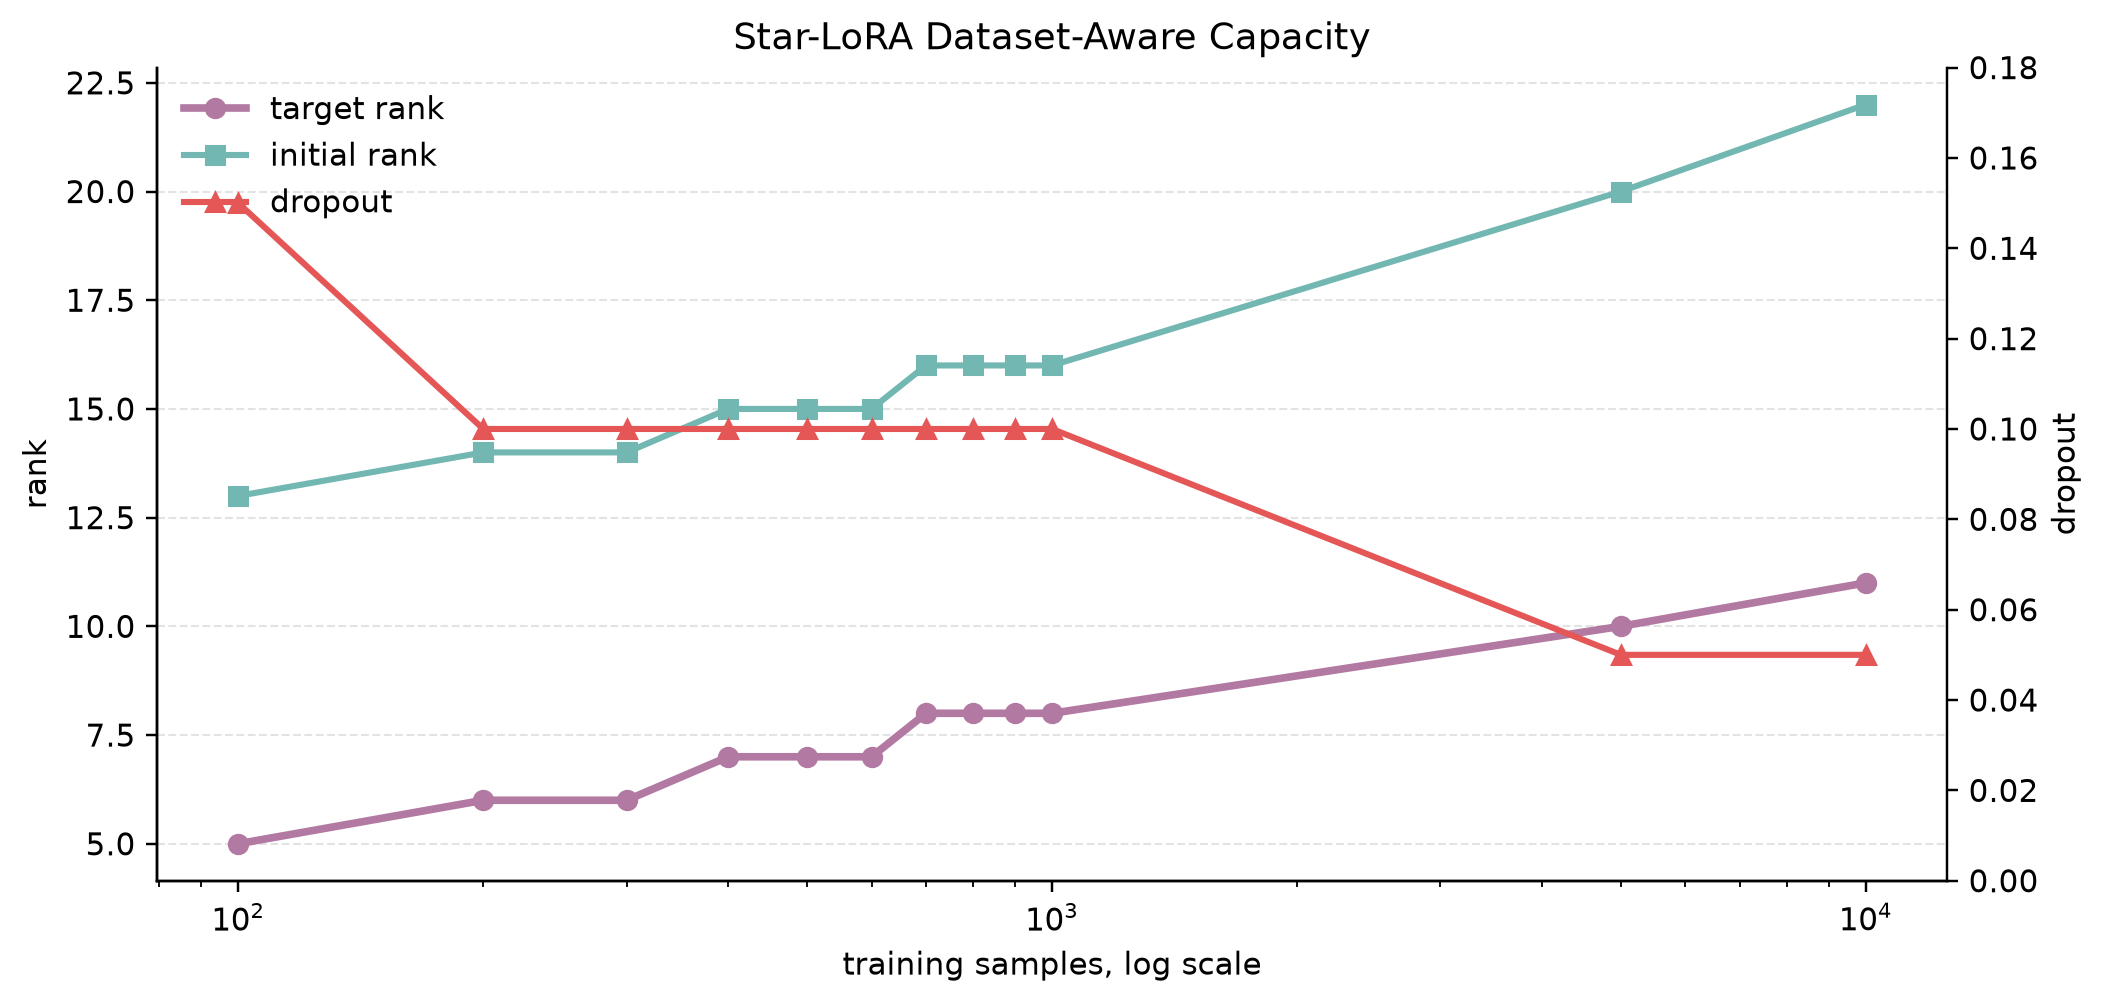
\includegraphics[width=0.93\linewidth]{figures/rank_policy.png}
\end{figure}
\end{frame}

\begin{frame}{Stability-Aware Importance Monitor}
\begin{figure}
    \centering
    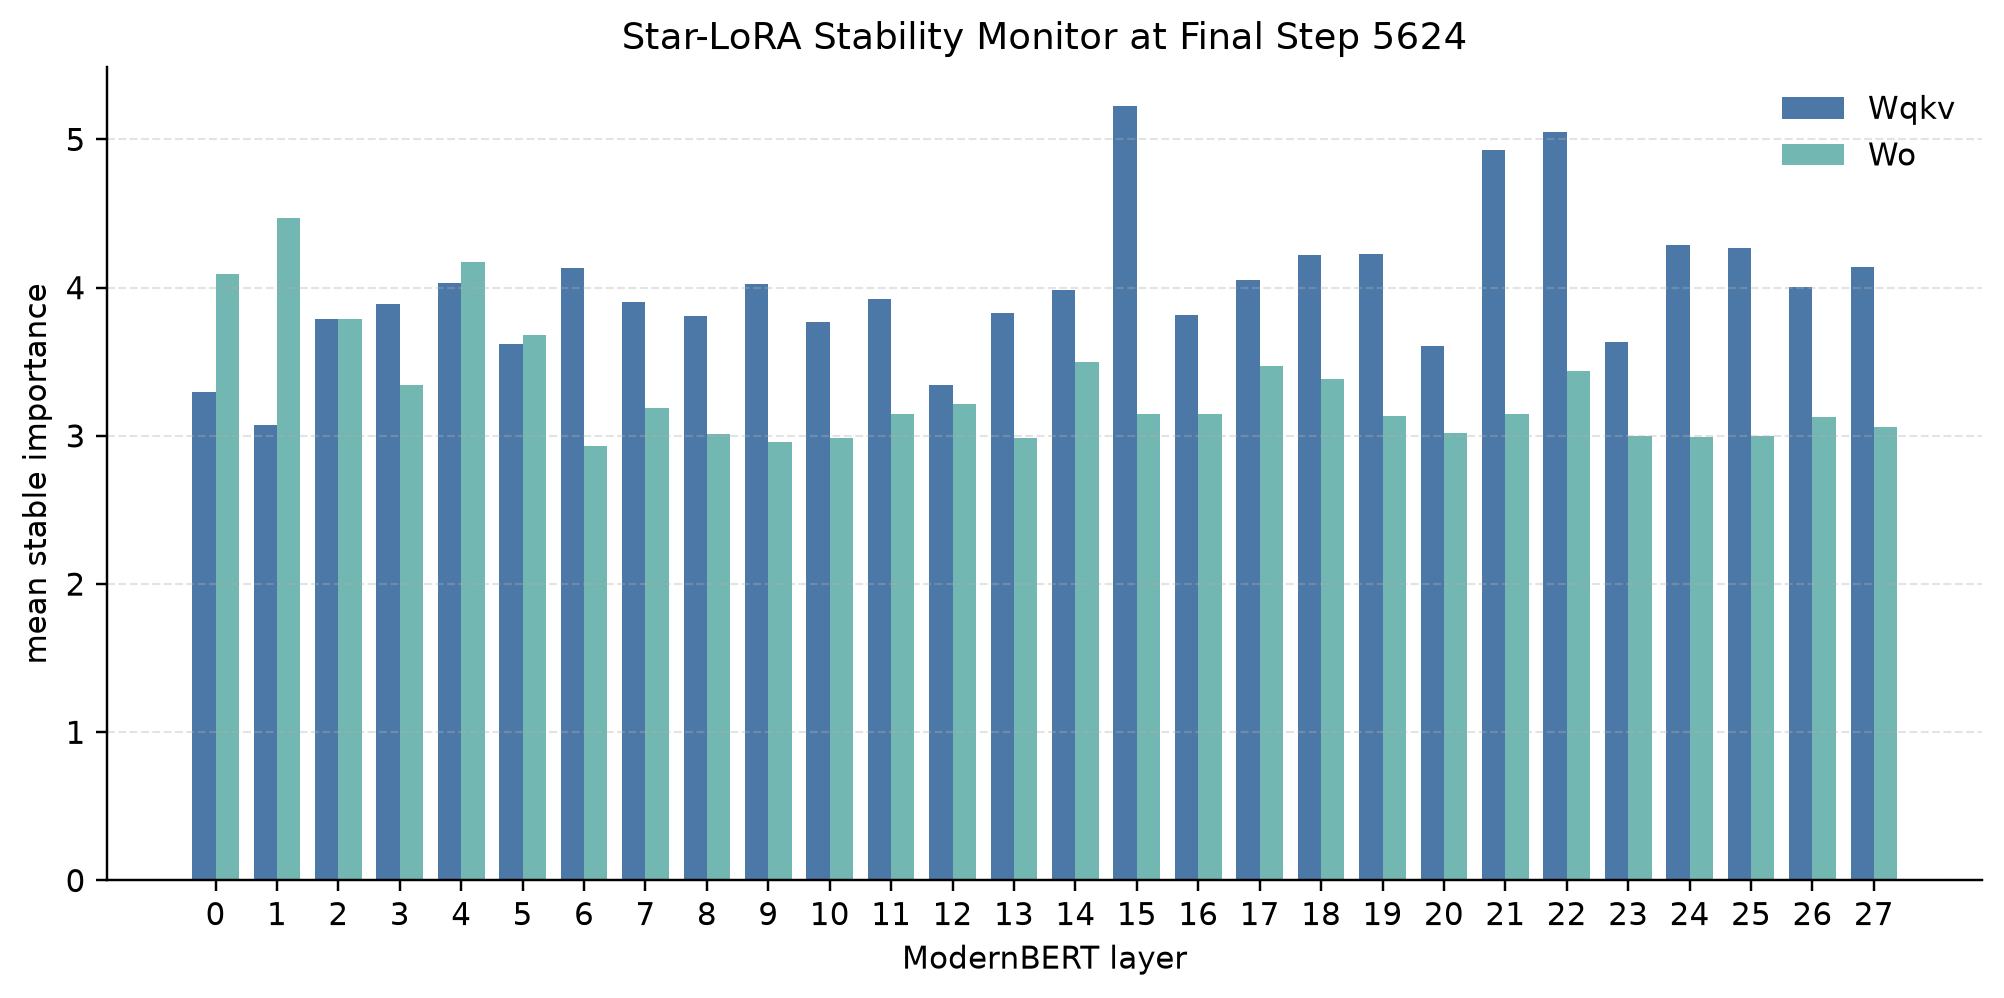
\includegraphics[width=0.93\linewidth]{figures/stability_by_layer.png}
\end{figure}

\vspace{-2pt}
\begin{itemize}
  \item The stability log makes layer-wise adapter importance inspectable after training.
  \item In the final Star-LoRA run, attention input projection \texttt{Wqkv} has higher mean stable importance than \texttt{Wo}.
\end{itemize}
\end{frame}
